%==============================================================================
%  MATH 231 -- Linear Algebra I (Queens College, Fall 2026)
%  HOMEWORK 4 -- Transformations, Determinants, Systems and Least Squares
%
%  STATUS: started 2026-11-05.  Due Sunday, November 29, 2026, 11:59 PM
%  (set by the instructor 2026-11-12).
%  Revised 2026-11-12: Part G (Gram-Schmidt and QR, S55-S58) removed, since
%  Part 11 will not be lectured before Midterm 2 (2026-11-24).  Its two
%  problems, with the part preamble, are now Problems 15-16 of the catalog in
%  plan/future_homework/ (gitignored).
%  Revised 2026-11-11 at the instructor's request:
%   - ROWS AND COLUMNS.  Students mixed up row and column vectors on HW3.
%     Convention now: x in R^n is a column; a bracket written across the line,
%     [a,b,c], is a ROW (in R^{1xn}); a column written across the line always
%     carries the transpose, [a,b,c]^T.  Stated in the "Rows and columns"
%     paragraph on page 1.  Every inline column in this file has \T; the only
%     bare brackets are genuine rows (F's preamble, F.2(b)).  Section 31.7's
%     "orthogonal to every row" is restated as r z = 0 (D preamble, D.1(c)).
%     NOTE: the lecture notes themselves use bare brackets for columns (Part 1
%     S5 says the bracket "never asserted a shape"); not changed there.
%   - PROBLEM A.4 (linear and affine maps) added, from the lecture just before
%     2026-11-11: linearity of maps/operators, C^infinity(R), affine maps, and
%     the 2x3 matrix [A : b] acting on [x,y,t]^T as A[x,y]^T + t b.  That
%     lecture has no notes file, so A.4 defines everything it uses.  It went
%     into Part A (not a new Part H) to keep the limit of 7 parts.
%
%  SCOPE.  This file covers the matrix unit, Parts 3-10:
%     MATH231_matrices_3_matrices_that_move_the_plane          (S15-S21)
%     MATH231_matrices_4_area_and_rotation                     (S22-S25)
%     MATH231_matrices_5_projections_and_direct_sums           (S26-S29)
%     MATH231_matrices_6_null_space_and_rank_nullity           (S30-S34)
%     MATH231_matrices_7_the_determinant                       (S35-S39)
%     MATH231_matrices_8_gaussian_elimination                  (S40-S45)
%     MATH231_matrices_9_least_squares                         (S46-S49)
%     MATH231_matrices_10_the_inverse_and_the_pseudoinverse    (S50-S54)
%  As of 2026-11-05 only Parts 1-5 had been lectured (through the Householder
%  reflector, Nov 3).  If topics are dropped from Parts 6-10, delete the
%  matching problems; the cross-references are listed below.
%
%  LIMITS SET BY THE INSTRUCTOR: at most 7 parts and at most 12 pages.  Since
%  Part G was removed it has 6 parts, A-F.
%  Every problem also has at most 7 lettered sub-parts, (a)-(g).
%
%  LAYOUT.  Six parts, one per topic, in lecture order:
%     A  Matrices that move the plane      S15-S21, S24-S25
%        + linear and affine maps (A.4)    lecture only, no notes file
%     B  Projections, reflections, direct sums   S26-S29
%     C  Determinants                      S22-S23, S35-S39
%     D  The null space and rank-nullity   S30-S34
%     E  Elimination and the inverse       S40-S45, S50-S53
%     F  Least squares and the pseudo-inverse    S46-S49, S54
%
%  CROSS-REFERENCES BETWEEN PROBLEMS (update them if a problem is cut):
%   - B.1(d) points at the matrices of A.1.
%   - B.3(b) uses the formula of B.1(c).
%   - C.1(c) uses R_{pi/3} from Part A's preamble.
%   - F.2(a) checks its identity on F.1.
%   - A.4(c) uses V_S from Part A's preamble; A.4(e) and (f) use the T of
%     A.4(c); A.4(e) uses the 3x3 block form of S17.4; A.4(f) uses R_{pi/4}.
%
%  FROM THE FUTURE-HOMEWORK CATALOG (plan/future_homework/, gitignored):
%   - A.1 is catalog Problem 5 ("A gallery of motions", was HW3 F.2), cut to
%     six matrices and now allowed to use determinants and S21.2.
%   - A.2 is catalog Problem 6 ("One motion after another", was HW3 F.3);
%     (d) and (e) are new (S24.6, S17.3-S17.4).
%   - B.1 merges catalog Problems 9 and 12 (building projection matrices;
%     projecting onto the all-ones vector).  B.1(d) is the rewrite of the old
%     G.3(e) that the catalog note asked for.
%   - Not used: catalog Problems 4, 7, 8, 10, 11 (their content is now proved
%     in the Part 3-5 lectures), 13-14 (the Hessian), and 1-3 (held back
%     from Homework 2).
%
%  MATERIAL NOT IN THE LECTURES, defined inside the problem that uses it:
%   - skew-symmetric matrices (C.3(b)), as in Homework 3;
%   - the mean of a list of numbers (B.1(e));
%   - linear maps, C^infinity(R), affine maps and [A : b] (A.4).
%
%  NUMBERS.  Every numerical answer was checked in exact arithmetic.  The
%  line-fit data of the lectures, (1,1), (2,2), (3,2), is deliberately NOT
%  used; F.1 uses (0,1), (1,3), (2,4), (3,4), whose best line is
%  y = 3/2 + t with residual [-1/2, 1/2, 1/2, -1/2].
%
%  WRITTEN ONLY.  There is no programming part.  Any NumPy companion belongs in
%  a separate, optional extra-credit assignment.
%
%  NUMBERING.  As in Homeworks 1-3: parts are lettered, problems numbered by
%  part.  Bare section numbers refer to the matrix unit, whose numbering runs
%  continuously through Parts 1-11.
%
%  NO ANSWER KEY, by design, as in Homeworks 1-3.
%
%  The submission path in the "What to submit" callout is homework/hw4/ in
%  the student repo.
%
%  Compile with pdflatex or tectonic (standard TeX Live packages only; uses
%  tikz for the house in A.2).
%==============================================================================

\documentclass[11pt]{article}

\usepackage[margin=1in]{geometry}
\usepackage{amsmath,amssymb}
\usepackage[dvipsnames]{xcolor}
\usepackage{enumitem}
\usepackage{booktabs}
\usepackage{array}
\usepackage[hidelinks]{hyperref}
\usepackage{titlesec}
\usepackage{needspace}
\usepackage{tikz}

%------------------------------------------------------------------ style ----
\titleformat{\section}{\large\bfseries\sffamily\color{RoyalBlue}}
                      {Part \thesection.}{0.6em}{}
\titleformat{\subsection}{\normalsize\bfseries\sffamily}{\thesubsection.}{0.5em}{}
\titlespacing*{\section}{0pt}{16pt}{7pt}

\renewcommand{\thesection}{\Alph{section}}

% Keeps long inline formulas from pushing a line into the margin.
\setlength{\emergencystretch}{3em}

% The problem heading is a line of its own, so that part (a) -- or the opening
% sentence -- always starts below it.  (An amsthm theorem cannot promise this: a
% list that opens the body runs its first item onto the heading line.)
\makeatletter
\newcounter{prob}[section]
\renewcommand{\theprob}{\thesection.\arabic{prob}}
\newenvironment{prob}[1][]
  {\par\addvspace{16pt plus 6pt minus 4pt}%
   \needspace{4\baselineskip}%
   \refstepcounter{prob}%
   \noindent\textbf{Problem~\theprob}%
   \if\relax\detokenize{#1}\relax\else\ (#1)\fi\textbf{.}%
   \par\nobreak\@afterindentfalse\@afterheading}
  {\par\addvspace{16pt plus 6pt minus 4pt}}
\makeatother

\newcommand{\hint}[1]{\par\smallskip\noindent
  {\small\sffamily\textcolor{RoyalBlue}{\textbf{Hint.}}\ #1}\par\smallskip}

% shaded call-out box.  The body is collected into a savebox first, because
% \colorbox needs its whole argument at once.
\definecolor{softbg}{HTML}{F2F6FA}
\newsavebox{\qcbox}
\newenvironment{callout}[1]
  {\par\medskip\needspace{5\baselineskip}%
   \begin{lrbox}{\qcbox}%
   \begin{minipage}{\dimexpr\textwidth-2\fboxsep-4pt}%
   \setlength{\parskip}{0.4em}%
   \textbf{\sffamily\color{RoyalBlue}#1}\par}
  {\end{minipage}\end{lrbox}%
   \begin{center}\colorbox{softbg}{\usebox{\qcbox}}\end{center}\medskip}

% The sub-part list used by every problem.
\newlist{parts}{enumerate}{1}
\setlist[parts]{label=\textbf{(\alph*)},leftmargin=2.6em,itemsep=5pt,topsep=5pt}
%--------------------------------------------------------------- notation ----
\newcommand{\R}{\mathbb{R}}
\newcommand{\vc}[1]{\mathbf{#1}}
\newcommand{\mt}[1]{\mathbf{#1}}          % matrices: bold upper case
\newcommand{\T}{^{\mathsf{T}}}            % transpose
\newcommand{\one}{\mathbf{1}}
\newcommand{\norm}[1]{\lVert #1\rVert}
\newcommand{\proj}[2]{\operatorname{proj}_{#1}(#2)}
\newcommand{\colsp}[1]{\operatorname{col}[#1]}
\newcommand{\rowsp}[1]{\operatorname{row}[#1]}
\newcommand{\nullsp}[1]{\operatorname{null}[#1]}
\newcommand{\xh}{\hat{\vc{x}}}
\DeclareMathOperator{\diagop}{diag}
\DeclareMathOperator{\rank}{rank}
\DeclareMathOperator{\nullity}{nullity}
\DeclareMathOperator{\spanop}{span}
\DeclareMathOperator{\adj}{adj}
\newenvironment{aug}[1]{\left[\begin{array}{#1}}{\end{array}\right]}

%--------------------------------------------------------- fill this in ------
\newcommand{\duedate}{Sunday, November 29, 2026, 11:59 PM}

\title{\vspace{-1.2cm}\textbf{\sffamily MATH 231 -- Linear Algebra I}\\[4pt]
       {\large\sffamily Homework 4 \textbullet\ Transformations, Determinants,
        Systems and Least Squares}\\[2pt]
       {\normalsize\sffamily Kiely Hall 326 \textbullet\
        Instructor: Kevin Bedoya}}
\author{}
\date{}

\begin{document}
\maketitle
\vspace{-1.6cm}

\noindent\textbf{Due:} \duedate.

\medskip
\begin{center}
\small
\renewcommand{\arraystretch}{1.08}
\begin{tabular}{@{}l l >{\raggedright\arraybackslash}p{12cm}@{}}
\toprule
\textbf{Matrix Unit} & \textbf{Sections} & \textbf{Topics} \\
\midrule
Part 3 & \S15--\S21 & a matrix from what it does; scaling, translation, shear; orthogonal matrices \\
Part 4 & \S22--\S25 & the $2\times2$ determinant and area; the rotation matrix; rotations of $\R^{3}$ \\
Part 5 & \S26--\S29 & projection matrices; reflections; the Householder reflector; the direct sum \\
Part 6 & \S30--\S34 & the null space; rank--nullity; $\rank(\mt{A}\T\mt{A})$; the $2\times2$ inverse \\
Part 7 & \S35--\S39 & cofactors; the Laplace expansion; principal minors; the laws D1--D10 \\
Part 8 & \S40--\S45 & row operations; Gaussian and Gauss--Jordan elimination; consistency \\
Part 9 & \S46--\S49 & least squares; the normal equations; fitting a line \\
Part 10 & \S50--\S54 & Cramer's rule; the inverse; the adjugate; the pseudo-inverse \\
Lecture & --- & linear maps and operators; $C^{\infty}(\R)$; affine maps and their matrix $[\,\mt{A}:\vc{b}\,]$ \\
\bottomrule
\end{tabular}
\end{center}

\noindent\textbf{Grading.} Every problem is worth the same number of points.

\smallskip
\noindent\textbf{Section numbers and notation.} A bare section number such as
\S28.4 refers to the matrix unit, whose numbering runs straight through
Parts 1--11. $\vc{e}_i$ is the standard basis vector with a $1$ in slot $i$.
For a matrix $\mt{A}$, $\colsp{\mt{A}}$, $\rowsp{\mt{A}}$ and $\nullsp{\mt{A}}$
are its column space, row space and null space.

\smallskip
\noindent\textbf{Rows and columns.} A vector $\vc{x}\in\R^{n}$ is a
\emph{column}, an $n\times1$ matrix. A \emph{row} vector is a $1\times n$
matrix, an element of $\R^{1\times n}$. A bracket written across the line is a
row, so a column written across the line carries a transpose:
$\vc{x}=[\,x_1,\dots,x_n\,]\T\in\R^{n}$. For example,
$[\,3,1\,]\in\R^{1\times2}$ is a row, while
$[\,3,1\,]\T=\left[\begin{smallmatrix}3\\1\end{smallmatrix}\right]\in\R^{2}$
is a column, and $\vc{u}\T\vc{v}$ is a number while $\vc{u}\vc{v}\T$ is a
matrix. Keep the two apart in your answers too: a column written across the
line needs its $\T$.

\smallskip
\noindent\textbf{On the proof problems} (A.1(e), A.3(a), (b), A.4(a), (b), (d)--(f),
B.2(a)--(c), B.3(b), C.3(b), (c), D.2(a)--(c), E.3(d), (e), and F.2(a)). None
of them requires a clever idea. Write down what you are assuming, justify each
step by naming the definition, law or theorem that licenses it, and end with a
sentence saying what you have shown. A chain of equalities with no words is not
a proof; neither is a paragraph of words with no computation.

\smallskip
\noindent\textbf{Collaboration} is encouraged --- work at a board together, argue
about the problems. What you submit must be written by you, in your own words.

\begin{callout}{What to submit}
Push your written work for Parts A--F to your own MATH 231 GitHub repository,
as a single PDF named \texttt{hw4.pdf} in a folder named \texttt{homework/hw4/}.
Handwritten and scanned or photographed is completely fine, as long as it is
legible and the pages are in order.

\textbf{PDF is the only accepted format.} A \texttt{.docx}, a \texttt{.jpg}, a
\texttt{.png}, a \texttt{.heic}, or a link to a file hosted somewhere else will
not be graded.

\textbf{Type Parts A--F up instead and you earn $+5$ points of extra credit on
this assignment.} Any typesetting system counts --- \LaTeX, Word's equation
editor, or anything else that produces readable mathematics --- and the extra
credit is for the whole of Parts A--F, not for typing up some of it. Sketches
may be drawn by hand and scanned into the PDF.
\end{callout}

\begin{callout}{Label every answer}
Label each answer with the number of the problem it answers --- \texttt{A.3(b)},
\texttt{E.2(d)} --- and put your answers \textbf{in the same order as they
appear in this assignment}. A grader who cannot tell which question a piece of
work belongs to cannot award it credit. You do not have to copy the question
out: write the label, then your work.
\end{callout}

%==============================================================================
\section{Matrices that move the plane; linear and affine maps}
%==============================================================================
\emph{Matrix Unit, \S15--\S21 and \S24--\S25.} Identify the point $(x,y)$ with
the column $[\,x,y\,]\T$. A matrix $\mt{M}\in\R^{2\times2}$ moves each point
$\vc{p}$ to $\mt{M}\vc{p}$, and its columns are the points to which it moves
$\vc{e}_1$ and $\vc{e}_2$ (the recipe of \S15.1). To move a polygon, list its
corners as the columns of a matrix $\mt{V}\in\R^{2\times k}$, compute the single
product $\mt{M}\mt{V}$, and join the moved corners in the same order. Doing
$\mt{B}$ first and then $\mt{A}$ is the single matrix $\mt{A}\mt{B}$ (\S15.4).
A square matrix $\mt{Q}$ is \textbf{orthogonal} if
$\mt{Q}\T\mt{Q}=\mt{Q}\mt{Q}\T=\mt{I}$ (\S20.6), and the $2\times2$ orthogonal
matrices are exactly the rotations $\left[\begin{smallmatrix}a&-c\\c&a\end{smallmatrix}\right]$
and the reflections $\left[\begin{smallmatrix}a&c\\c&-a\end{smallmatrix}\right]$
with $a^{2}+c^{2}=1$ (\S21.2). In the angle form of \S24.2 and \S24.7,
\[
  \mt{R}_\theta=\begin{bmatrix}\cos\theta&-\sin\theta\\\sin\theta&\cos\theta\end{bmatrix},
  \qquad
  \mt{F}_\theta=\begin{bmatrix}\cos\theta&\sin\theta\\\sin\theta&-\cos\theta\end{bmatrix}:
\]
$\mt{R}_\theta$ rotates counterclockwise by $\theta$, and $\mt{F}_\theta$
reflects across the line through the origin at angle $\theta/2$.
Two shapes are used below: the unit square $S$ and the standard triangle
$\Delta$, with corner matrices
$\mt{V}_S=\left[\begin{smallmatrix}0&1&1&0\\0&0&1&1\end{smallmatrix}\right]$ and
$\mt{V}_\Delta=\left[\begin{smallmatrix}0&1&0\\0&0&1\end{smallmatrix}\right]$.
Draw every sketch on graph paper, or on hand-drawn axes with the grid marked,
with the original shape and the moved shape on the same axes.

%------------------------------------------------------------------------------
\begin{prob}[A gallery of motions]
Here are six matrices:
\[
  \mt{M}_1=\begin{bmatrix}2&0\\0&3\end{bmatrix},\quad
  \mt{M}_2=\begin{bmatrix}0&1\\1&0\end{bmatrix},\quad
  \mt{M}_3=\begin{bmatrix}0&-1\\1&0\end{bmatrix},
\]
\[
  \mt{M}_4=\begin{bmatrix}1&2\\0&1\end{bmatrix},\quad
  \mt{M}_5=\frac12\begin{bmatrix}1&1\\1&1\end{bmatrix},\quad
  \mt{M}_6=\frac{1}{\sqrt2}\begin{bmatrix}1&-1\\1&1\end{bmatrix}.
\]
\begin{parts}
  \item For each $\mt{M}_i$, compute $\mt{M}_i\mt{V}_S$, sketch $S$ and its
        image, and say what $\mt{M}_i$ does to the square: a stretch (by how
        much in each direction), a reflection (across which line), a rotation
        (by which angle, and which way), a shear (which way), or a collapse
        onto a line (which line).
  \item For each $\mt{M}_i$, read the area of the image of $S$ off your sketch,
        and compute $\det\mt{M}_i$. Check that the area is
        $\lvert\det\mt{M}_i\rvert$ (\S23.4). Which of the six reverse
        orientation?
  \item Which of the six are orthogonal? Write each one that is as
        $\mt{R}_\theta$ or $\mt{F}_\theta$ for a specific angle $\theta$.
  \item Find the matrix that moves $\Delta$ onto the triangle with corners
        $(0,0)$, $(3,1)$, $(1,2)$, and the one that moves $\Delta$ onto the
        triangle with corners $(0,0)$, $(-1,2)$, $(4,0)$. Use a determinant to
        find the area of each of the two triangles.
  \item Prove that no $2\times2$ matrix moves $\Delta$ onto the triangle with
        corners $(1,1)$, $(2,1)$, $(1,2)$. Then write a $3\times3$ matrix, in
        homogeneous coordinates (\S17.3), that does.
\end{parts}
\end{prob}

%------------------------------------------------------------------------------
\begin{prob}[One motion after another]
The house below has corners $(0,0)$, $(2,0)$, $(2,2)$, $(1,3)$, $(0,2)$, taken
in that order. Let
\[
  \mt{V}_H=\begin{bmatrix}0&2&2&1&0\\0&0&2&3&2\end{bmatrix},
  \qquad
  \mt{R}=\begin{bmatrix}0&-1\\1&0\end{bmatrix},
  \qquad
  \mt{F}=\begin{bmatrix}1&0\\0&-1\end{bmatrix},
\]
so that $\mt{R}$ is the quarter turn counterclockwise and $\mt{F}$ is the
reflection across the $x$-axis.
\begin{center}
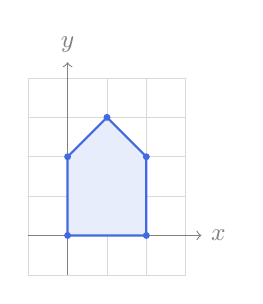
\begin{tikzpicture}[scale=0.5]
  \draw[gray!30,very thin] (-1,-1) grid (3,4);
  \draw[->,gray] (-1,0) -- (3.4,0) node[right] {\small $x$};
  \draw[->,gray] (0,-1) -- (0,4.4) node[above] {\small $y$};
  \draw[thick,RoyalBlue,fill=RoyalBlue!12]
    (0,0) -- (2,0) -- (2,2) -- (1,3) -- (0,2) -- cycle;
  \foreach \p in {(0,0),(2,0),(2,2),(1,3),(0,2)} \fill[RoyalBlue] \p circle (2.5pt);
\end{tikzpicture}
\end{center}
\begin{parts}
  \item Compute $\mt{R}\mt{V}_H$ and sketch the turned house.
  \item Compute $\mt{F}(\mt{R}\mt{V}_H)$, which turns the house and then
        reflects it, and $\mt{R}(\mt{F}\mt{V}_H)$, which reflects it and then
        turns it. Sketch both. Do they agree?
  \item Compute the single matrices $\mt{F}\mt{R}$ and $\mt{R}\mt{F}$, and check
        that $(\mt{F}\mt{R})\mt{V}_H=\mt{F}(\mt{R}\mt{V}_H)$. Each of
        $\mt{F}\mt{R}$ and $\mt{R}\mt{F}$ is a reflection: write each as
        $\mt{F}_\theta$, and name the line it reflects across.
  \item Since $\mt{R}=\mt{R}_{\pi/2}$, use \S24.6 to write $\mt{R}^{2}$,
        $\mt{R}^{3}$ and $\mt{R}^{4}$ as rotations $\mt{R}_\theta$ without
        multiplying. Then check your answer for $\mt{R}^{2}$ by multiplying.
  \item Write the $3\times3$ matrix, in homogeneous coordinates
        (\S17.3--\S17.4), that first turns the house by $\mt{R}$ and then
        translates it by $[\,3,1\,]\T$. Apply it to all five corners with one
        matrix product, and sketch the result.
\end{parts}
\end{prob}

%------------------------------------------------------------------------------
\begin{prob}[Orthogonal matrices]
\begin{parts}
  \item Let $\mt{Q}_1$ and $\mt{Q}_2$ be orthogonal $n\times n$ matrices. Prove
        that $\mt{Q}_1\mt{Q}_2$ is orthogonal, naming the laws of \S8.4 you use.
  \item Using the angle-addition formulas
        $\cos(\alpha-\beta)=\cos\alpha\cos\beta+\sin\alpha\sin\beta$ and
        $\sin(\alpha-\beta)=\sin\alpha\cos\beta-\cos\alpha\sin\beta$, prove that
        $\mt{F}_\alpha\mt{F}_\beta=\mt{R}_{\alpha-\beta}$: two reflections make
        a rotation. Check it for $\alpha=\pi/2$ and $\beta=0$ by multiplying.
  \item Find every $2\times2$ orthogonal matrix whose first column is
        $[\,\tfrac{5}{13},\tfrac{12}{13}\,]\T$. For the rotation, give
        $\cos\theta$ and $\sin\theta$. For the reflection, find a nonzero vector
        on its mirror line and check that the matrix leaves it where it is.
  \item Let $\mt{M}=\mt{R}_x(\tfrac{\pi}{2})\,\mt{R}_z(\tfrac{\pi}{2})$, with
        \[
          \mt{R}_x(\theta)=\begin{bmatrix}1&0&0\\0&\cos\theta&-\sin\theta\\0&\sin\theta&\cos\theta\end{bmatrix},
          \qquad
          \mt{R}_z(\theta)=\begin{bmatrix}\cos\theta&-\sin\theta&0\\\sin\theta&\cos\theta&0\\0&0&1\end{bmatrix}
        \]
        the rotations of \S25.1--\S25.2. Compute $\mt{M}$ and
        $\mt{M}\T\mt{M}$. Find every vector $\vc{v}\in\R^{3}$ with
        $\mt{M}\vc{v}=\vc{v}$, and compute $\mt{M}^{3}$. ($\mt{M}$ is the
        rotation of space by $2\pi/3$ about the line you found.)
\end{parts}
\end{prob}

%------------------------------------------------------------------------------
\begin{prob}[Linear and affine maps]
\emph{From the lecture on linear and affine maps.} Functions are added and
scaled point by point: $(f+g)(x)=f(x)+g(x)$ and $(\alpha f)(x)=\alpha f(x)$.
$C^{\infty}(\R)$ is the set of functions $f:\R\to\R$ that have derivatives of
every order, $f',f'',f''',\dots$. A map $T$ whose inputs are vectors of
$\R^{n}$, or functions in $C^{\infty}(\R)$, is \textbf{linear} if
$T(u+v)=T(u)+T(v)$ and $T(\alpha u)=\alpha\,T(u)$ for all inputs $u,v$ and
every number $\alpha$. For
$\mt{A}\in\R^{2\times2}$ and $\vc{b}\in\R^{2}$, the \textbf{affine map}
$T(\vc{p})=\mt{A}\vc{p}+\vc{b}$ applies $\mt{A}$ to the point $\vc{p}$ and then
shifts it by $\vc{b}$. Its matrix is the $2\times3$ matrix
$[\,\mt{A}:\vc{b}\,]$, whose first two columns are those of $\mt{A}$ and whose
third column is $\vc{b}$:
\[
  [\,\mt{A}:\vc{b}\,]\begin{bmatrix}x\\y\\t\end{bmatrix}
  =\mt{A}\begin{bmatrix}x\\y\end{bmatrix}+t\,\vc{b},
  \qquad\text{so}\qquad
  T\bigl([\,x,y\,]\T\bigr)=[\,\mt{A}:\vc{b}\,]\,[\,x,y,1\,]\T.
\]
\begin{parts}
  \item Let $L:C^{\infty}(\R)\to C^{\infty}(\R)$ be $L(f)=f''-3f'+2f$. Prove
        that $L$ is linear, naming the rules of differentiation you use.
        Compute $L(e^{x})$, $L(e^{2x})$ and $L(x)$, and then use linearity
        alone, with no more differentiation, to find
        $L(5e^{x}-2e^{2x}+4x)$.
  \item Prove that every linear map $T$ sends $\vc{0}$ to $\vc{0}$. Then
        prove that none of these three maps is linear, by finding specific
        inputs at which one of the two properties fails: $g:\R\to\R$,
        $g(x)=3x+2$; $h:\R^{2}\to\R$, $h\bigl([\,x,y\,]\T\bigr)=xy$; and
        $N:C^{\infty}(\R)\to C^{\infty}(\R)$, $N(f)=f\,f'$. ($h$ and $N$ do
        send $\vc{0}$ to $\vc{0}$, so for them that test is not enough.)
  \item Let $\mt{A}=\left[\begin{smallmatrix}1&-1\\1&1\end{smallmatrix}\right]$,
        $\vc{b}=[\,2,-1\,]\T$ and $T(\vc{p})=\mt{A}\vc{p}+\vc{b}$. Write
        $[\,\mt{A}:\vc{b}\,]$. Move the unit square $S$ with one product: append
        a row of $1$s to $\mt{V}_S$, multiply by $[\,\mt{A}:\vc{b}\,]$ on the
        left, and sketch $S$ and $T(S)$. Compare the area of $T(S)$ with
        $\lvert\det\mt{A}\rvert$.
  \item Prove that an affine map $T(\vc{p})=\mt{A}\vc{p}+\vc{b}$ is linear if
        and only if $\vc{b}=\vc{0}$. Then prove that the map
        $\R^{3}\to\R^{2}$, $\vc{u}\mapsto[\,\mt{A}:\vc{b}\,]\,\vc{u}$, is linear
        for every $\mt{A}$ and $\vc{b}$, naming the laws of \S8.4 you use. (So
        $T$ is a linear map one dimension up, used only on the inputs with
        $t=1$; compare the remark in \S17.3.)
  \item Let $S(\vc{p})=\mt{C}\vc{p}+\vc{d}$ be a second affine map. Prove that
        doing $T$ and then $S$ is the affine map with matrix
        $[\,\mt{C}\mt{A}:\mt{C}\vc{b}+\vc{d}\,]$. The product
        $[\,\mt{C}:\vc{d}\,][\,\mt{A}:\vc{b}\,]$ of two $2\times3$ matrices is
        not defined; the $3\times3$ matrices of \S17.4 fix this. For the $T$
        of (c) and
        $\mt{C}=\left[\begin{smallmatrix}1&0\\0&-1\end{smallmatrix}\right]$,
        $\vc{d}=[\,0,1\,]\T$, check that
        $\left[\begin{smallmatrix}\mt{C}&\vc{d}\\\vc{0}\T&1\end{smallmatrix}\right]
        \left[\begin{smallmatrix}\mt{A}&\vc{b}\\\vc{0}\T&1\end{smallmatrix}\right]$
        has $[\,\mt{C}\mt{A}:\mt{C}\vc{b}+\vc{d}\,]$ as its top two rows.
  \item For the $T$ of (c), find the point $\vc{c}$ with $T(\vc{c})=\vc{c}$,
        and prove that $T(\vc{p})=\vc{c}+\mt{A}(\vc{p}-\vc{c})$ for every
        $\vc{p}\in\R^{2}$. Check that $\mt{A}=\sqrt2\,\mt{R}_{\pi/4}$: $T$
        turns the plane by $\pi/4$ about $\vc{c}$ and stretches every distance
        from $\vc{c}$ by $\sqrt2$.
\end{parts}
\end{prob}

%==============================================================================
\section{Projections, reflections, and the direct sum}
%==============================================================================
\emph{Matrix Unit, \S26--\S29.} For a nonzero $\vc{u}\in\R^{n}$, the projection
matrix onto the line $\spanop\{\vc{u}\}$ is
$\mt{P}_{\vc{u}}=\vc{u}\vc{u}\T/\vc{u}\T\vc{u}$, and
$\mt{P}_{\vc{u}}\vc{v}=\proj{\vc{u}}{\vc{v}}=\frac{\vc{u}\T\vc{v}}{\vc{u}\T\vc{u}}\,\vc{u}$
(\S26.2). A square matrix $\mt{P}$ is a \textbf{projection matrix} if
$\mt{P}^{2}=\mt{P}$ (\S27.2), and an \textbf{orthogonal projection matrix} if
also $\mt{P}\T=\mt{P}$ (\S27.4). By the theorem of \S27.4, for an orthogonal
projection matrix the leftover $\vc{v}-\mt{P}\vc{v}$ is orthogonal to every
vector of $\colsp{\mt{P}}$. The reflection across $\spanop\{\vc{u}\}$ is
$2\mt{P}_{\vc{u}}-\mt{I}$ (\S28.4). For $\vc{u}\in\R^{2}$ not on the negative
$x$-axis, the \textbf{Householder reflector} is
\[
  \mt{H}=2\vc{v}\vc{v}\T-\mt{I}_2,
  \qquad
  \vc{v}=\frac{\vc{m}}{\norm{\vc{m}}},
  \qquad
  \vc{m}=\tfrac12\bigl(\vc{u}+\norm{\vc{u}}\,\vc{e}_1\bigr),
\]
and $\mt{H}\vc{u}=\norm{\vc{u}}\,\vc{e}_1$ (\S28.5--\S28.6). If $U$ and $W$ are
subspaces of $\R^{n}$, then $\R^{n}=U\oplus W$, the \textbf{direct sum}, means
that every vector of $\R^{n}$ can be written in exactly one way as
$\vc{u}+\vc{w}$ with $\vc{u}\in U$ and $\vc{w}\in W$. By the theorem of
\S29.3, this holds if and only if every vector is such a sum and
$U\cap W=\{\vc{0}\}$.

%------------------------------------------------------------------------------
\begin{prob}[Building projection matrices]
\begin{parts}
  \item Compute $\mt{P}_{\vc{u}}$, with exact fractions, for
        $\vc{u}=[\,1,-2\,]\T$, $[\,2,-1,2\,]\T$ and $[\,1,2,2\,]\T$. For each, check
        that $\mt{P}_{\vc{u}}$ is symmetric and that
        $\mt{P}_{\vc{u}}\vc{u}=\vc{u}$, and give its rank.
  \item With $\vc{u}=[\,1,2,2\,]\T$ and $\vc{v}=[\,3,0,3\,]\T$, compute
        $\mt{P}_{\vc{u}}\vc{v}$ and check it against the formula for
        $\proj{\vc{u}}{\vc{v}}$. Then compute
        $(\mt{I}-\mt{P}_{\vc{u}})\vc{v}$ and check that it is orthogonal to
        $\vc{u}$.
  \item Let $\vc{u}=[\,\cos\theta,\sin\theta\,]\T$. Show that
        $\mt{P}_{\vc{u}}=\left[\begin{smallmatrix}\cos^{2}\theta&\cos\theta\sin\theta\\
        \cos\theta\sin\theta&\sin^{2}\theta\end{smallmatrix}\right]$, and that
        $2\mt{P}_{\vc{u}}-\mt{I}=\mt{F}_{2\theta}$, the reflection across the
        line at angle $\theta$. Use $\cos2\theta=2\cos^{2}\theta-1=1-2\sin^{2}\theta$
        and $\sin2\theta=2\sin\theta\cos\theta$.
  \item Which matrix of Problem A.1 is $\mt{P}_{\vc{u}}$ for
        $\vc{u}=[\,1,1\,]\T$? Which is $2\mt{P}_{\vc{u}}-\mt{I}$ for the same
        $\vc{u}$?
  \item Let $\one=[\,1,1,1,1\,]\T\in\R^{4}$. Write out $\mt{P}_{\one}$, and
        compute $\mt{P}_{\one}\vc{x}$ and $(\mt{I}-\mt{P}_{\one})\vc{x}$ for
        $\vc{x}=[\,4,7,1,8\,]\T$. Then show that for every $\vc{x}\in\R^{4}$,
        every entry of $\mt{P}_{\one}\vc{x}$ equals the \textbf{mean}
        $\tfrac14(x_1+x_2+x_3+x_4)$ of the entries of $\vc{x}$.
\end{parts}
\end{prob}

%------------------------------------------------------------------------------
\begin{prob}[Projections that are not orthogonal]
In (a)--(c), $\mt{P}$ is an $n\times n$ matrix with $\mt{P}^{2}=\mt{P}$.
\begin{parts}
  \item Prove that $\mt{P}\T$ is also a projection matrix. Name the law of
        \S8.4 you use.
  \item Prove that a vector $\vc{v}\in\R^{n}$ lies in $\colsp{\mt{P}}$ if and
        only if $\mt{P}\vc{v}=\vc{v}$.
  \item Suppose also that $\mt{P}\T=\mt{P}$. Prove that
        $\norm{\mt{P}\vc{v}}\le\norm{\vc{v}}$ for every $\vc{v}\in\R^{n}$.
        \hint{Write $\vc{v}=\mt{P}\vc{v}+(\vc{v}-\mt{P}\vc{v})$, and use the
        theorem of \S27.4 and the Pythagorean identity.}
  \item Let $\mt{P}=\left[\begin{smallmatrix}1&2\\0&0\end{smallmatrix}\right]$. Check that
        $\mt{P}^{2}=\mt{P}$ and that $\mt{P}$ is not symmetric. Describe
        $\colsp{\mt{P}}$, and the set of vectors that $\mt{P}$ sends to
        $\vc{0}$, as lines. Compare $\norm{\mt{P}\vc{e}_2}$ with
        $\norm{\vc{e}_2}$.
  \item With the same $\mt{P}$, split $\vc{x}=[\,3,1\,]\T$ as
        $\mt{P}\vc{x}+(\mt{I}-\mt{P})\vc{x}$ (\S29.5). Are the two pieces
        orthogonal? Is $\norm{\vc{x}}^{2}=\norm{\mt{P}\vc{x}}^{2}+\norm{(\mt{I}-\mt{P})\vc{x}}^{2}$?
\end{parts}
\end{prob}

%------------------------------------------------------------------------------
\begin{prob}[The Householder reflector, and direct sums]
\begin{parts}
  \item Let $\vc{u}=[\,8,15\,]\T$. Compute $\vc{m}$, $\vc{v}$ and
        $\mt{H}=2\vc{v}\vc{v}\T-\mt{I}$ with exact entries. Check that
        $\mt{H}\vc{u}=[\,17,0\,]\T$, that the first column of $\mt{H}$ is
        $\vc{u}/\norm{\vc{u}}$, and that $\mt{H}^{2}=\mt{I}$.
  \item Let $\vc{u}=r\,[\,\cos\theta,\sin\theta\,]\T$ with $r>0$ and
        $-\pi<\theta<\pi$. Prove that the Householder reflector of $\vc{u}$ is
        $\mt{F}_\theta$, so its mirror is the line at angle $\theta/2$, halfway
        between $\vc{u}$ and the positive $x$-axis.
        \hint{The half-angle identities $1+\cos\theta=2\cos^{2}\frac{\theta}{2}$
        and $\sin\theta=2\sin\frac{\theta}{2}\cos\frac{\theta}{2}$ give
        $\vc{m}=r\cos\frac{\theta}{2}\,\vc{w}$, where
        $\vc{w}=[\,\cos\frac{\theta}{2},\sin\frac{\theta}{2}\,]\T$.
        Then use B.1(c).}
  \item Let $U=\spanop\{[\,1,0\,]\T\}$ and $W=\spanop\{[\,1,2\,]\T\}$, subspaces of
        $\R^{2}$. Use the theorem of \S29.3 to show that $\R^{2}=U\oplus W$, and
        split $\vc{x}=[\,4,6\,]\T$ into its piece in $U$ and its piece in $W$.
        Find the $2\times2$ matrix $\mt{P}$ that sends every $\vc{x}$ to its
        piece in $U$, check that $\mt{P}^{2}=\mt{P}$, and say whether $\mt{P}$
        is an orthogonal projection matrix.
  \item Let $W=\{\vc{x}\in\R^{3}:x_1+x_2+x_3=0\}$, a subspace of $\R^{3}$.
        Show that $\R^{3}=\spanop\{[\,1,1,0\,]\T\}\oplus W$, and split
        $[\,3,1,2\,]\T$ into its two pieces. Then show that $\R^{3}$ is
        \emph{not} $\spanop\{[\,1,-1,0\,]\T\}\oplus W$.
\end{parts}
\end{prob}

%==============================================================================
\section{Determinants}
%==============================================================================
\emph{Matrix Unit, \S22--\S23 and \S35--\S39.} The parallelogram with sides the
columns of $\mt{A}\in\R^{2\times2}$ has area $\lvert\det\mt{A}\rvert$ (\S23.4),
and $\mt{A}$ multiplies the area of every region by $\lvert\det\mt{A}\rvert$
(\S23.6). For $\mt{A}\in\R^{n\times n}$, the minor $M_{ij}$ is the determinant
of $\mt{A}$ with row $i$ and column $j$ deleted, and the cofactor is
$C_{ij}=(-1)^{i+j}M_{ij}$ (\S35). Then $\det\mt{A}=\sum_{j}a_{1j}C_{1j}$, and
expanding along any other row or column gives the same number (\S36).

\needspace{9\baselineskip}
\noindent The laws of \S38.1 are:
\begin{center}
\small
\renewcommand{\arraystretch}{1.15}
\begin{tabular}{@{}l >{\raggedright\arraybackslash}p{6.2cm} l >{\raggedright\arraybackslash}p{6.2cm}@{}}
\textbf{D1} & $\det\mt{I}_n=1$ &
\textbf{D6} & two equal rows give $\det\mt{A}=0$ \\
\textbf{D2} & $\det\mt{A}\T=\det\mt{A}$ &
\textbf{D7} & $\det$ is linear in each row separately \\
\textbf{D3} & a zero row gives $\det\mt{A}=0$ &
\textbf{D8} & adding a multiple of one row to another leaves $\det$ unchanged \\
\textbf{D4} & scaling one row by $\alpha$ scales $\det$ by $\alpha$; so
  $\det(\alpha\mt{A})=\alpha^{n}\det\mt{A}$ &
\textbf{D9} & $\det(\mt{A}\mt{B})=\det\mt{A}\,\det\mt{B}$ \\
\textbf{D5} & swapping two rows changes the sign &
\textbf{D10} & $\det\mt{A}\neq0\iff\rank\mt{A}=n\iff\nullsp{\mt{A}}=\{\vc{0}\}$ \\
\end{tabular}
\end{center}
By D2, every law about rows is also a law about columns. The determinant of a
triangular matrix is the product of its diagonal entries (\S39.1). Keeping the
rows \emph{and} the columns numbered by a set $S\subseteq\{1,\dots,n\}$ gives a
principal submatrix, whose determinant is a \textbf{principal minor}; for
$S=\{1,\dots,k\}$ it is the $k$-th \textbf{leading principal minor} $\Delta_k$
(\S37.1). A symmetric $\mt{A}$ is \textbf{positive definite} if
$\vc{x}\T\mt{A}\vc{x}>0$ for every $\vc{x}\neq\vc{0}$, which happens exactly
when $\Delta_1,\dots,\Delta_n$ are all positive (Sylvester's criterion, \S37.3).

%------------------------------------------------------------------------------
\begin{prob}[Area]
\begin{parts}
  \item Find the area of the parallelogram with sides $[\,4,1\,]\T$ and
        $[\,2,5\,]\T$, and of the triangle with corners $(1,1)$, $(5,2)$ and
        $(3,6)$.
  \item Find every number $k$ for which the triangle with corners $(0,0)$,
        $(3,1)$ and $(k,2)$ has area $4$.
  \item A region of the plane has area $5$. Let
        $\mt{M}=\left[\begin{smallmatrix}3&1\\2&4\end{smallmatrix}\right]$. Find the area of its
        image under $\mt{M}$, under $\mt{M}^{2}$, under
        $\mt{R}_{\pi/3}\mt{M}$, and under $\tfrac12\mt{M}$, naming the facts of
        \S22 and \S23.6 you use.
\end{parts}
\end{prob}

%------------------------------------------------------------------------------
\begin{prob}[Computing determinants]
Let
\[
  \mt{B}=\begin{bmatrix}2&-1&3\\1&4&0\\-2&1&5\end{bmatrix},
  \qquad
  \mt{A}=\begin{bmatrix}1&0&2&0\\3&1&0&2\\0&0&4&0\\2&0&1&3\end{bmatrix},
  \qquad
  \mt{T}_k=\begin{bmatrix}1&k&0\\k&1&k\\0&k&1\end{bmatrix}.
\]
\begin{parts}
  \item Compute $\det\mt{B}$ by expanding along the first row, and again by
        expanding down the third column.
  \item Compute $\det\mt{A}$, expanding along whichever row or column makes the
        work shortest (\S36.4).
  \item Compute $\det\mt{B}$ a third time: reduce $\mt{B}$ to an upper
        triangular matrix by row operations, record the effect of each one on
        the determinant (\S38.3), and finish with \S39.1.
  \item Find every number $k$ for which $\det\mt{T}_k=0$. For the positive
        one, find a nonzero vector $\vc{x}$ with $\mt{T}_k\vc{x}=\vc{0}$.
\end{parts}
\end{prob}

%------------------------------------------------------------------------------
\begin{prob}[Laws, two proofs, and positive definite matrices]
\begin{parts}
  \item Let $\mt{A}$ be $3\times3$ with $\det\mt{A}=4$. Find
        $\det(2\mt{A})$, $\det(-\mt{A})$, $\det(\mt{A}^{3})$ and
        $\det(\mt{A}\T\mt{A})$. Then find the determinant of the matrix obtained
        from $\mt{A}$ by (i) swapping rows $1$ and $3$; (ii) adding $5$ times
        row $2$ to row $1$; (iii) tripling row $2$ and then swapping rows $1$
        and $2$. Name the law used each time.
  \item A square matrix $\mt{K}$ is \textbf{skew-symmetric} if
        $\mt{K}\T=-\mt{K}$. Prove that if $\mt{K}$ is $n\times n$ and
        skew-symmetric and $n$ is odd, then $\det\mt{K}=0$. Check it on
        $\left[\begin{smallmatrix}0&1&-2\\-1&0&3\\2&-3&0\end{smallmatrix}\right]$,
        and show that the skew-symmetric
        $\left[\begin{smallmatrix}0&1\\-1&0\end{smallmatrix}\right]$ has
        nonzero determinant.
  \item Prove that
        \[
          \det\begin{bmatrix}1&1&1\\a&b&c\\a^{2}&b^{2}&c^{2}\end{bmatrix}
          =(b-a)(c-a)(c-b),
        \]
        and deduce that this determinant is $0$ exactly when two of $a,b,c$
        are equal.
        \hint{Subtract column $1$ from columns $2$ and $3$ (D8 for columns),
        expand along the first row, and factor.}
  \item Let $\mt{S}=\left[\begin{smallmatrix}2&-1&0\\-1&2&-1\\0&-1&2\end{smallmatrix}\right]$.
        Find all seven principal minors of $\mt{S}$ and its three leading
        principal minors. Is $\mt{S}$ positive definite?
  \item For $\mt{A}=\left[\begin{smallmatrix}1&3\\3&4\end{smallmatrix}\right]$, compute $\Delta_1$
        and $\Delta_2$, and find a vector $\vc{x}$ with
        $\vc{x}\T\mt{A}\vc{x}<0$.
        \hint{Look at the vector used in the proof of Sylvester's criterion in
        \S37.3.}
\end{parts}
\end{prob}

%==============================================================================
\section{The null space and rank--nullity}
%==============================================================================
\emph{Matrix Unit, \S30--\S34.} The \textbf{null space} of
$\mt{A}\in\R^{m\times n}$ is $\nullsp{\mt{A}}=\{\vc{x}\in\R^{n}:\mt{A}\vc{x}=\vc{0}\}$,
a subspace of $\R^{n}$, and its dimension is the \textbf{nullity} (\S31). The
matrix has \textbf{full column rank} if $\rank\mt{A}=n$, \textbf{full row rank}
if $\rank\mt{A}=m$, and \textbf{full rank} if $\rank\mt{A}=\min(m,n)$ (\S30.1).
The rank--nullity theorem says $\rank\mt{A}+\nullity\mt{A}=n$ (\S32). If
$\vc{x}_p$ is one solution of $\mt{A}\vc{x}=\vc{b}$, the solutions are exactly
$\vc{x}_p+\vc{z}$ with $\vc{z}\in\nullsp{\mt{A}}$ (\S31.6). If $\vc{r}$ is a
row of $\mt{A}$ and $\vc{z}\in\nullsp{\mt{A}}$, then $\vc{r}\vc{z}=0$, so
$\vc{z}$ is orthogonal to the column $\vc{r}\T$ (\S31.7), and
$\rank(\mt{A}\T\mt{A})=\rank\mt{A}=\rank\mt{A}\T$ (\S33). For square
$\mt{A}$, a subspace $W$ is \textbf{invariant} under $\mt{A}$ if
$\mt{A}\vc{w}\in W$ for every $\vc{w}\in W$ (\S30.4). If $ad-bc\neq0$, then
$\left[\begin{smallmatrix}a&b\\c&d\end{smallmatrix}\right]^{-1}
=\frac{1}{ad-bc}\left[\begin{smallmatrix}d&-b\\-c&a\end{smallmatrix}\right]$,
and if $ad-bc=0$ there is no inverse (\S34).

%------------------------------------------------------------------------------
\begin{prob}[Null spaces, rank and nullity]
Let
\[
  \mt{A}_1=\begin{bmatrix}1&2&3\\2&4&6\end{bmatrix},\quad
  \mt{A}_2=\begin{bmatrix}1&0&2\\0&1&-1\\1&1&1\end{bmatrix},\quad
  \mt{A}_3=\begin{bmatrix}1&1\\1&-1\\2&0\end{bmatrix},\quad
  \mt{A}_4=\begin{bmatrix}1&2&0&1\\0&0&1&3\end{bmatrix}.
\]
\begin{parts}
  \item For each $\mt{A}_i$, write $\nullsp{\mt{A}_i}$ as the span of as few
        vectors as possible, or show that it is $\{\vc{0}\}$, and give the
        nullity.
  \item Give the rank of each $\mt{A}_i$ and check rank--nullity. Say whether
        each has full rank, full column rank, full row rank, or none of these.
  \item Check that $\vc{r}\vc{z}=0$ for every row $\vc{r}$ of $\mt{A}_2$ and
        every vector $\vc{z}$ you used to span $\nullsp{\mt{A}_2}$.
  \item Find every solution of $\mt{A}_2\vc{x}=[\,3,1,4\,]\T$ in the form
        $\vc{x}_p+\vc{z}$, $\vc{z}\in\nullsp{\mt{A}_2}$. Then show that
        $\mt{A}_2\vc{x}=[\,1,1,1\,]\T$ has no solution.
  \item A matrix $\mt{A}\in\R^{6\times9}$ has rank $4$. Find $\nullity\mt{A}$,
        $\rank\mt{A}\T$, $\nullity\mt{A}\T$, $\rank(\mt{A}\T\mt{A})$ and
        $\rank(\mt{A}\mt{A}\T)$, naming the result you use each time.
\end{parts}
\end{prob}

%------------------------------------------------------------------------------
\begin{prob}[Proofs, invariant lines, and the $2\times2$ inverse]
\begin{parts}
  \item Let $\mt{A}\in\R^{m\times n}$ and $\mt{B}\in\R^{p\times m}$. Prove that
        $\nullsp{\mt{A}}\subseteq\nullsp{\mt{B}\mt{A}}$. Then prove that if
        $\nullsp{\mt{B}}=\{\vc{0}\}$, then
        $\nullsp{\mt{B}\mt{A}}=\nullsp{\mt{A}}$.
  \item Let $\mt{A}\in\R^{m\times n}$ and $\mt{B}\in\R^{n\times p}$. Prove that
        $\colsp{\mt{A}\mt{B}}\subseteq\colsp{\mt{A}}$, and deduce that
        $\rank(\mt{A}\mt{B})\le\rank\mt{A}$. Then use the first statement of
        (a), applied to the product $\mt{A}\mt{B}$, together with rank--nullity,
        to show that $\rank(\mt{A}\mt{B})\le\rank\mt{B}$.
  \item Let $\mt{A}$ be $n\times n$. Prove that $\nullsp{\mt{A}}$ and
        $\colsp{\mt{A}}$ are invariant under $\mt{A}$. Then find every line
        through the origin that is invariant under
        $\left[\begin{smallmatrix}2&1\\0&3\end{smallmatrix}\right]$.
  \item For which numbers $k$ is $\mt{B}_k=\left[\begin{smallmatrix}k&4\\1&k\end{smallmatrix}\right]$
        invertible? For $k=3$, find $\mt{B}_3^{-1}$ and use it to solve
        $\mt{B}_3\vc{x}=[\,1,2\,]\T$. For $k=2$, find $\nullsp{\mt{B}_2}$ and
        $\colsp{\mt{B}_2}$.
\end{parts}
\end{prob}

%==============================================================================
\section{Elimination and the inverse}
%==============================================================================
\emph{Matrix Unit, \S40--\S45 and \S50--\S53.} The elementary row operations
are \textbf{(E1)} swap two rows, \textbf{(E2)} scale a row by a nonzero
number, \textbf{(E3)} add a multiple of one row to another. They do not change
the solutions of a system (\S40.3), and each one is multiplication on the left
by the \textbf{elementary matrix} obtained by doing it to $\mt{I}$ (\S40.4).
Row-echelon form is defined in \S42.5 and reduced row-echelon form (RREF) in
\S43.1. By \S43.4, the columns of $\mt{A}$ in the pivot positions of its RREF
form a basis of $\colsp{\mt{A}}$, and setting one free variable to $1$ and the
others to $0$, for each free variable in turn, gives a basis of
$\nullsp{\mt{A}}$. A system is consistent exactly when elimination produces no
row $[\,0\ \cdots\ 0\mid c\,]$ with $c\neq0$ (\S44.3).

A matrix $\mt{A}\in\R^{n\times n}$ is \textbf{invertible} if there is a
$\mt{B}$ with $\mt{A}\mt{B}=\mt{B}\mt{A}=\mt{I}$ (\S51.1). Gauss--Jordan
elimination turns $[\,\mt{A}\mid\mt{I}\,]$ into $[\,\mt{I}\mid\mt{A}^{-1}\,]$
(\S51.4). The \textbf{adjugate} $\adj\mt{A}$ is the transpose of the matrix of
cofactors, and $\mt{A}^{-1}=\frac{1}{\det\mt{A}}\adj\mt{A}$ (\S52). If
$\det\mt{A}\neq0$, \textbf{Cramer's rule} gives the solution of
$\mt{A}\vc{x}=\vc{b}$ as $x_i=\det\mt{A}_i(\vc{b})/\det\mt{A}$, where
$\mt{A}_i(\vc{b})$ is $\mt{A}$ with column $i$ replaced by $\vc{b}$ (\S50.1).
The laws of \S53.1 are \textbf{I1} $(\mt{A}^{-1})^{-1}=\mt{A}$,
\textbf{I2} $(\mt{A}\mt{B})^{-1}=\mt{B}^{-1}\mt{A}^{-1}$,
\textbf{I3} $(\mt{A}\T)^{-1}=(\mt{A}^{-1})\T$,
\textbf{I4} $(\alpha\mt{A})^{-1}=\alpha^{-1}\mt{A}^{-1}$,
\textbf{I5} $\det(\mt{A}^{-1})=1/\det\mt{A}$ and
\textbf{I6} $(\mt{A}^{k})^{-1}=(\mt{A}^{-1})^{k}$.

%------------------------------------------------------------------------------
\begin{prob}[Elimination, step by step]
\begin{parts}
  \item Solve the system
        \[
          x_1+2x_2+x_3=1,\qquad 2x_1+5x_2+3x_3=3,\qquad -x_1+x_2+4x_3=6
        \]
        by Gaussian elimination and back substitution, writing down each row
        operation. Then read off the determinant of the coefficient matrix
        $\mt{A}$ from the pivots (\S42.6).
  \item Write the elementary matrix of each row operation you used in (a).
        Check that their product, in the right order, times $\mt{A}$ is the
        upper triangular matrix you reached.
  \item Solve $\mt{L}\vc{x}=[\,4,5,3\,]\T$ by forward substitution (\S41.2),
        where $\mt{L}=\left[\begin{smallmatrix}2&0&0\\1&3&0\\-1&2&1\end{smallmatrix}\right]$.
\end{parts}
\end{prob}

%------------------------------------------------------------------------------
\begin{prob}[Reduced row-echelon form, bases, and consistency]
Let
\[
  \mt{A}=\begin{bmatrix}1&2&0&1&-1\\2&4&1&4&1\\1&2&1&3&2\end{bmatrix}.
\]
\begin{parts}
  \item Bring $\mt{A}$ to reduced row-echelon form, naming each row operation.
        Mark the pivots, and list the pivot variables and the free variables.
  \item Use \S43.4 to give a basis of $\colsp{\mt{A}}$ made of columns of
        $\mt{A}$, and a basis of $\nullsp{\mt{A}}$. Give the rank and the
        nullity, and check rank--nullity.
  \item Write each non-pivot column of $\mt{A}$ as a combination of the pivot
        columns of $\mt{A}$, and check one of them by computing.
  \item Find a condition on $b_1,b_2,b_3$ that holds exactly when
        $\mt{A}\vc{x}=[\,b_1,b_2,b_3\,]\T$ is consistent. Then find every solution
        of $\mt{A}\vc{x}=[\,2,5,3\,]\T$, and show that
        $\mt{A}\vc{x}=[\,1,1,1\,]\T$ has none.
\end{parts}
\end{prob}

%------------------------------------------------------------------------------
\begin{prob}[The inverse]
Let
\[
  \mt{M}=\begin{bmatrix}1&2&0\\0&1&3\\2&4&1\end{bmatrix},
  \qquad
  \mt{N}=\begin{bmatrix}2&0&1\\1&1&0\\0&3&1\end{bmatrix}.
\]
\begin{parts}
  \item Find $\mt{M}^{-1}$ by Gauss--Jordan elimination, and check that
        $\mt{M}\mt{M}^{-1}=\mt{I}$.
  \item Find $\mt{N}^{-1}$ by the adjugate, and check that
        $\mt{N}\mt{N}^{-1}=\mt{I}$.
  \item Use Cramer's rule to find $x_2$ alone in $\mt{N}\vc{x}=[\,1,3,5\,]\T$.
        Then confirm it with $\mt{N}^{-1}$ from (b).
  \item Let $\mt{A},\mt{B},\mt{C}$ be invertible $n\times n$ matrices. Prove
        that $(\mt{A}\mt{B}\mt{C})^{-1}=\mt{C}^{-1}\mt{B}^{-1}\mt{A}^{-1}$,
        naming the laws of \S8.4 and \S53.1 you use. Then prove that if
        $\mt{A}$ is invertible and $\mt{A}\mt{B}=\mt{A}\mt{C}$, then
        $\mt{B}=\mt{C}$.
  \item Let $\mt{A}$ be $n\times n$ with $\mt{A}^{2}=\mt{0}$. Prove that
        $\mt{A}$ is not invertible, and that $\mt{I}-\mt{A}$ is invertible with
        $(\mt{I}-\mt{A})^{-1}=\mt{I}+\mt{A}$. Check both statements on
        $\mt{A}=\left[\begin{smallmatrix}1&-1\\1&-1\end{smallmatrix}\right]$.
\end{parts}
\end{prob}

%==============================================================================
\section{Least squares and the pseudo-inverse}
%==============================================================================
\emph{Matrix Unit, \S46--\S49 and \S54.} A \textbf{least-squares solution} of
$\mt{A}\vc{x}=\vc{b}$ is a vector $\xh$ that makes $\norm{\mt{A}\vc{x}-\vc{b}}^{2}$
as small as possible (\S47.1). These are exactly the solutions of the
\textbf{normal equations} $\mt{A}\T\mt{A}\,\xh=\mt{A}\T\vc{b}$, which say that
the residual $\vc{b}-\mt{A}\xh$ is orthogonal to every column of $\mt{A}$
(\S47.2--\S47.3). The normal equations always have a solution, and it is unique
exactly when $\mt{A}$ has full column rank (\S49.1--\S49.2). To fit the line
$y=c_0+c_1t$ to data points $(t_i,y_i)$, row $i$ of $\mt{A}$ is the row vector $[\,1,t_i\,]$
and $\vc{b}$ lists the $y_i$ (\S49.4). The \textbf{pseudo-inverse} is
$\mt{A}^{+}=(\mt{A}\T\mt{A})^{-1}\mt{A}\T$ if $\mt{A}$ has independent columns
(\S54.2), and $\mt{A}^{+}=\mt{A}\T(\mt{A}\mt{A}\T)^{-1}$ if $\mt{A}$ has
independent rows, in which case $\mt{A}^{+}\vc{b}$ is the shortest solution of
$\mt{A}\vc{x}=\vc{b}$ (\S54.3). For any $\mt{A}$, $\mt{A}^{+}$ is the one matrix
$\mt{X}$ with
\textbf{(MP1)} $\mt{A}\mt{X}\mt{A}=\mt{A}$,
\textbf{(MP2)} $\mt{X}\mt{A}\mt{X}=\mt{X}$,
\textbf{(MP3)} $(\mt{A}\mt{X})\T=\mt{A}\mt{X}$ and
\textbf{(MP4)} $(\mt{X}\mt{A})\T=\mt{X}\mt{A}$ (\S54.4).

%------------------------------------------------------------------------------
\begin{prob}[Fitting a line]
The four data points are $(0,1)$, $(1,3)$, $(2,4)$ and $(3,4)$.
\begin{parts}
  \item Write the system $\mt{A}\vc{x}=\vc{b}$, with $\vc{x}=[\,c_0,c_1\,]\T$,
        that says the line $y=c_0+c_1t$ passes through all four points. Show by
        elimination that it has no solution.
  \item Form $\mt{A}\T\mt{A}$ and $\mt{A}\T\vc{b}$, solve the normal equations,
        and write down the best line.
  \item Compute the residual $\vc{r}=\vc{b}-\mt{A}\xh$, check that
        $\mt{A}\T\vc{r}=\vc{0}$, and find the sum of the squared errors. Sketch
        the four points, the line, and the four vertical segments whose lengths
        are the entries of $\vc{r}$.
  \item Compute $\mt{A}^{+}=(\mt{A}\T\mt{A})^{-1}\mt{A}\T$. Check that
        $\mt{A}^{+}\mt{A}=\mt{I}_2$ and that $\mt{A}^{+}\vc{b}=\xh$.
\end{parts}
\end{prob}

%------------------------------------------------------------------------------
\begin{prob}[Pythagoras, shortest solutions, and Moore--Penrose]
\begin{parts}
  \item Let $\xh$ be a least-squares solution of $\mt{A}\vc{x}=\vc{b}$. Prove
        that $\norm{\vc{b}}^{2}=\norm{\mt{A}\xh}^{2}+\norm{\vc{b}-\mt{A}\xh}^{2}$.
        Check it on Problem F.1.
  \item Use \S54.3 to find the shortest solution $\vc{x}^{+}$ of
        $x_1+2x_2+2x_3=9$. Check that $\vc{x}^{+}$ is orthogonal to every vector
        of the null space of the $1\times3$ matrix $[\,1,2,2\,]$, and compare its length with that of the
        solution $[\,9,0,0\,]\T$.
  \item The matrix $\mt{A}$ below has neither independent columns nor
        independent rows:
        \[
          \mt{A}=\begin{bmatrix}2&4\\1&2\end{bmatrix},
          \qquad
          \mt{X}=\frac{1}{25}\begin{bmatrix}2&1\\4&2\end{bmatrix}.
        \]
        Check that $\mt{X}$ satisfies MP1--MP4, so $\mt{X}=\mt{A}^{+}$. Show that $\mt{A}\mt{X}$ and
        $\mt{X}\mt{A}$ are the projection matrices $\mt{P}_{\vc{y}}$ and
        $\mt{P}_{\vc{z}}$ of \S26.2 for $\vc{y}=[\,2,1\,]\T$ and
        $\vc{z}=[\,1,2\,]\T$.
  \item With $\mt{A}$ from (c) and $\vc{b}=[\,5,0\,]\T$, show that the normal
        equations have infinitely many solutions, and find them all. Show that
        $\mt{A}^{+}\vc{b}$ is one of them, and that it is shorter than the
        least-squares solution $[\,2,0\,]\T$.
\end{parts}
\end{prob}

\bigskip
\noindent\rule{\textwidth}{0.4pt}

\smallskip
\noindent{\small Questions about any problem here belong in the class Discord,
where everyone can see the answer. Questions that are specific to your own work
--- ``is my proof of D.2(b) valid?'' --- are better brought to office hours,
Thursdays 3:00--4:00 PM in Kiely Hall 508. Please email ahead.}

\end{document}
